%!TEX root = ../NCVC2.tex

\mysection{NC生成}

\vspace*{1.5zh}
 通常のNC生成(標準生成)では輪郭パスは生成されませんので \menu{形状加工生成} を選択してください.
ダイアログは図\ref{fig:make} のように標準生成と変わりありません.
切削条件ファイルを指定しOKボタンを押すと,

\begin{figure}[H]
\centering
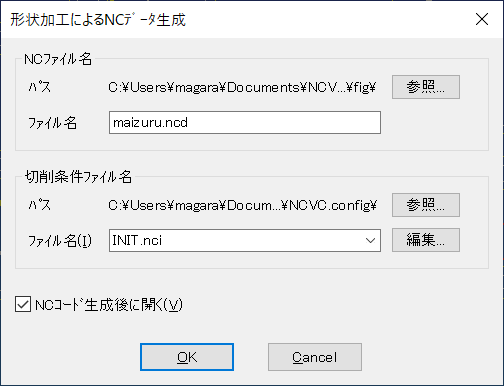
\includegraphics[scale=0.7]{No5/fig/dialog.png}
\caption{オフセット交点除去の確認ダイアログ}
\label{fig:make}
\end{figure}

 図\ref{fig:simu} のように生成できました.
標準生成と大きく異なるのは,部品の切り出し等を考慮して必ず内側の図形集合から切削されるようなパスを生成することです.
シミュレーション結果でよく確認してから切削を始めてください.

\begin{figure}[H]
\centering
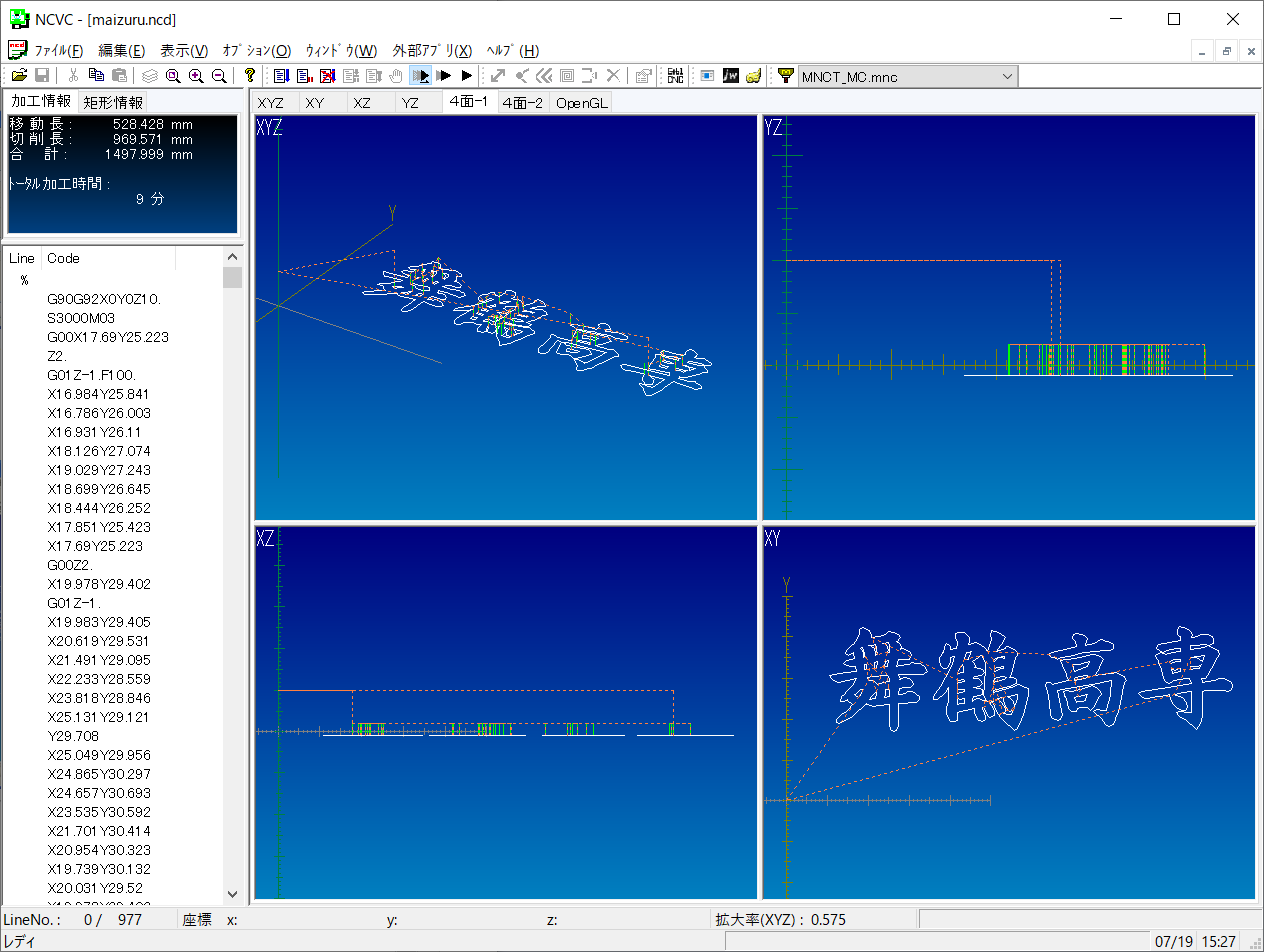
\includegraphics[scale=0.5]{No5/fig/maizuru.png}
\caption{シミュレーション画面}
\label{fig:simu}
\end{figure}
